\documentclass{webofc}

\usepackage{caption}
\usepackage{listings}
\usepackage[draft]{minted}
\usepackage[caption=false]{subfig}
\usepackage{hyperref}
\usepackage{graphicx}
%\usepackage{subcaption}
\usepackage{tikz}

% For arxiv we need to have next
%%%\usepackage{subcaption}
%\usepackage[draft]{minted}
%\usepackage[caption=false]{subfig}

\usepackage{minted}
\captionsetup{justification=raggedright,singlelinecheck=false,format=hang,labelfont=bf}
\usepackage[varg]{txfonts}   % Web of Conferences font
\newminted{cpp}{gobble=2, numbersep=3pt, escapeinside=||, xleftmargin=8mm, framesep=5mm, frame=leftline, baselinestretch=1, fontsize=\scriptsize, linenos=false}
\newmintinline{cpp}{}

\usetikzlibrary{shadows, arrows, fit, positioning, matrix, shapes}
\usetikzlibrary{decorations.markings}

% Define colors
\definecolor{my_yellow}{RGB}{255, 253, 217}
\definecolor{my_orange}{RGB}{255, 127, 0}
\definecolor{my_lightblue}{RGB}{105, 186, 249}
\definecolor{my_purple}{RGB}{150, 154, 219}
\definecolor{my_green}{RGB}{90, 194, 160}

% Define block styles  
\tikzset {
  bigbox/.style = {draw, thick, fill=gray!10, rounded corners, rectangle},
  box/.style = {draw, thick, minimum height=0.8cm, minimum width=1.5cm, rounded corners, rectangle, fill=white, anchor=south},
  model/.style = {draw, thick, fill=white, text centered, minimum height=3em, minimum width=4em, rounded corners, drop shadow},
  user/.style = {draw, thick, ellipse, fill=white, text centered, minimum height=3em, minimum width=5em, drop shadow},
  line/.style = {->, thick, color=black, shorten <=2pt, shorten >=2pt, >=stealth'},
  dashed/.style = {->, dash pattern=on 3pt off 3pt, color=gray, shorten <=2pt, shorten >=2pt, >=stealth'},
  plain/.style = {minimum width=1em},
  %\draw [line, ->] (m1.north) ++(-15pt,-1pt) arc [start angle=-140, end angle=-400, radius=20pt] node[midway] {$T_{M_1}$} ;
  % This works around an issue with node[midway] http://tex.stackexchange.com/questions/38763/how-to-place-a-node-in-the-middle-of-an-arc                
  arcnode/.style 2 args={
    decoration={
                 raise=#1,             
                 markings,   
                 mark=at position 0.5 with {\node[inner sep=0] {#2};}
            },
            postaction={decorate}
    }
}

% Define the layers to draw the diagram
\pgfdeclarelayer{background}
\pgfdeclarelayer{foreground}
\pgfsetlayers{background,main,foreground}

% Draw background
\newcommand{\background}[5]{%
  \begin{pgfonlayer}{background}
    % Left-top corner of the background rectangle
    \path (#1.west |- #2.north)+(-0.5,0.25) node (a1) {};
    % Right-bottom corner of the background rectanle
    \path (#3.east |- #4.south)+(+0.5,-0.25) node (a2) {};
    % Draw the background
    \path[rounded corners, draw=black!50, dashed, name=box]
      (a1) rectangle (a2);
    \path (a1 |- a2) -- (a2) node[midway,below] {\large\textit{#5}};
  \end{pgfonlayer}}

% Define a circled symbol command used throughout the thesis.
\newcommand*\circled[1]{\tikz[baseline=(char.base)]{
            \node[shape=circle,draw,inner sep=2pt] (char) {#1};}}
            
\begin{document}
%
\title{Extending ROOT through Modules}
%
% subtitle is optionnal
%
%%%\subtitle{Do you have a subtitle?\\ If so, write it here}

\author{\firstname{Oksana} \lastname{Shadura}\inst{1}\fnsep\thanks{\email{oksana.shadura@cern.ch}},
\firstname{Brian Paul }\lastname{Bockelman}\inst{1}\fnsep\thanks{\email{bbockelm@cse.unl.edu}},
\firstname{Vassil} \lastname{Vassilev}\inst{2}\fnsep\thanks{\email{vvasilev@cern.ch}}
        % etc.
}

\institute{University of Nebraska Lincoln, 1400 R St, Lincoln, NE 68588, United States
\and
           Princeton University, Princeton, New Jersey 08544, United States
          }

\abstract{%
The ROOT software framework is foundational for the HEP ecosystem, providing multiple capabilities such as I/O, a C++ interpreter, GUI, and math libraries. It uses object-oriented concepts and build-time components to layer between them. We believe that a new layering formalism will benefit the ROOT user community.

We present the modularization strategy for ROOT which aims to build upon the existing source components, making available the dependencies and other metadata outside of the build system, and allow post-install additions on top of existing installation as well as in the ROOT runtime environment. Components can be grouped into packages and made available from repositories in order to provide a post-install step of missing packages. This feature implements a mechanism for the more comprehensive software ecosystem and makes it available even from a minimal ROOT installation.  As part of this work, we have reduced inter-component dependencies in order to improve maintainability.

The modularization effort draws inspiration from similar efforts in the Java, Python, and Swift ecosystems. Keeping aligned with modern C++, this strategy relies on forthcoming features such as C++ modules. We hope formalizing the component layer provides simpler ROOT installs, improves extensibility, and decreases the complexity of embedding ROOT in other ecosystems.
}
%https://www.overleaf.com/2984268478jqhnpvkswcxn
\maketitle
%
\section{Introduction}

One of the advantages of object-oriented systems is the ability to have abstraction layers that provide separation between the user interfaces and implementations. Ultimately, it is an important tool to help to scale projects to larger code bases. Another technique for scaling projects is to use a modularization. Modularisation provides a grouping of functionality into distinct units with clear points of interaction.  While ROOT \cite{root} has a strong history in object-oriented programming, it doesn’t have as a strong a concept of modular components.  Thus, we propose to add new concepts to the ROOT ecosystem:
\begin{enumerate}
\item \textit{Component}: A set of interdependent classes implementing coherent functionality and providing well-defined APIs. A \textit{library} could be defined as a component or set of related components that expose functionality and which can be invoked by a program or another library.
\item \textit{Package}: A distinct, self-describing resource (file, URL) that provide one or more components (such as a library and associated non-code resources).
\item \textit{Package database}: A record of all packages currently available in a ROOT installation.
\item \textit{Package manager}: An actor that can locate and install packages into a ROOT installation from a package reference (such as a package URL), along with their transitive dependencies.
\end{enumerate}

Similar to ROOT, other large object-oriented software systems consist of a number of interdependent and loosely-coupled classes and are mostly organized as a set of libraries and build targets.  In these cases, classes are often used as the lowest level of granularity and can serve as a unit of software modularization.

In ecosystems such as Java, Python, and C++, a further package structure can allow software developers to organize their programs into components. A good organization of classes into identifiable and collaborating packages simplifies the understanding and the maintenance of the software. Yet another technique to improve the quality of the software modularization is to provide technical mechanisms for encouraging coders to utilize these package structures.

% Since we address large software systems as the ROOT framework, consisting of a substantial number of classes and packages, we consider that packages are the units of software modularization.

\section{Motivation}

Software modularization defines a way of grouping functionalities. It outlines groups in the form of components, which identify a particular piece of functionality that solves a specific problem.  Often, it provides a way for coders to carefully specify the visibility of interfaces and differentiate this between inside the package and outside.  In general, modularization helps reducing management, coordination and development costs. We aim to define a set of mechanisms that enable a modular version of ROOT, centered around C++ modules \cite{rootcxxmodules} and the concept of software packages.

ROOT libraries have a very complex set of interdependencies. By introducing a component layer on top of these libraries, we provide better boundaries between components, allowing ROOT to scale as a project. We hope this can also make it easier for external communities to develop packages on top of ROOT and easily distribute them -- without needing to get their work into ROOT's official codebase. 

 A first step is to define a \textit{minimal ROOT} package, removing as many dependencies as possible, until only the simplest user functionality remains; we decided the minimal functionality should effectively be the I/O libraries and C++ interpreter. By having a smaller size and set of external dependency, we increase the chances that its functionality can be embedded in other contexts and enables ROOT users to interact with the broader data science ecosystem.

Packages and package management provides a mechanism for ROOT users to socialize and reuse projects built on top of ROOT. We aim to help make ROOT more flexible and open it to the new customers. This feature would allow ROOT to  serve as a community nexus. In particular, it provides the ROOT team with an improved mechanism to say “no” to new components within the ROOT source itself as users can directly share their packages among each other or in a conventional store such as GitHub.

\section{ROOT components and packages}

The ROOT code \cite{rootgit} is organized into a set of sub-directories per component, with the exception of the ROOT Core library, which has a more complex structure of subfolders.

A component is a single unit of code distribution or set of classes for a framework or an application that is built and ready to be shipped. Another C++ module \cite{cxxmodules} or another component can import it with a hook, such as an ``include" keyword in case of headers (or the ``import" keyword in case of C++ modules).

% TODO(brian): I don't understand what the next few sentences mean - commenting out
% Oksana: agree, could be dropped!

%This model requires a few definitions:
%\begin{enumerate}
%\item Define components as a ROOT installation “unit". It could also be defined as a component or package with the single component inside which is distributed and maintained through 'standard' ROOT (i.e., lives in root.git). \cite{rootgit}

%\item Every facility is provided by exactly one component.
%\end{enumerate}

As an example, Figure 1 shows how a package can be created based on multiple components. Here, a hypothetical \textit{ROOT-ML package} consists of the TMVA (``Toolkit for Multivariate Data Analysis") component and ROOT RDataframe as its dependencies.

The ROOT modularization work is well-aligned with the effort to integrate C++ modules work going \cite{rootcxxmodules} in ROOT. C++ modules provide a simple way to produce software libraries with improved compile-time scalability and management of the API of a library. C++ modules improve encapsulation and outline a clear relationship between public and private part of the code, splitting the two into implementation and interface.
For ROOT, we are working on an ecosystem to improve versioning and binary distribution.

\begin{figure}[!h]
  \centering
    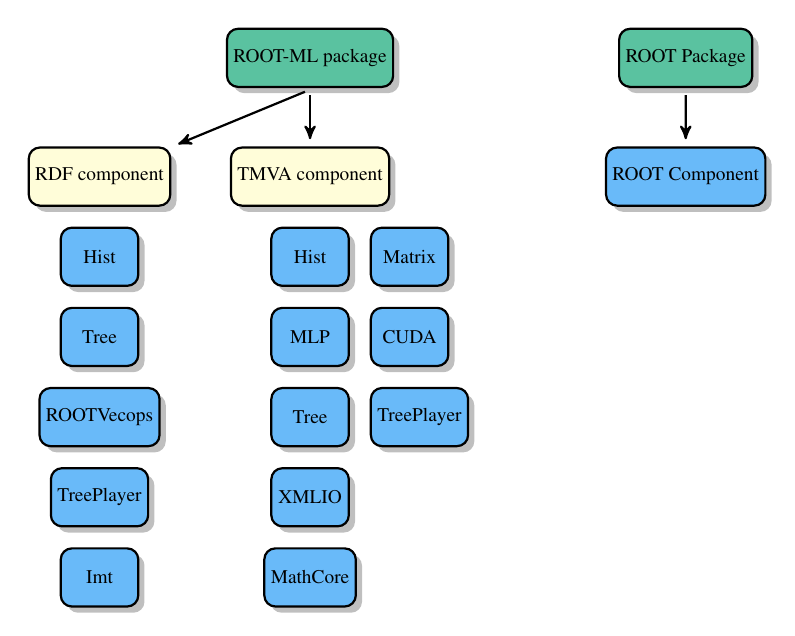
\begin{tikzpicture}[outer sep=0.05cm, node distance=0.8cm, scale=0.7, transform shape]
    \node[model, fill=my_green, name=rootml] (rootml) {ROOT-ML package};   
    \node[model, fill=my_green, name=pkg, right=4cm of rootml] (pkg) {ROOT Package};
    \node[model, fill=my_lightblue, name=component, below=1cm of pkg] (component) {ROOT Component};
    \node[model, fill=my_yellow, name=tmva, below=1cm of rootml] (tmva) {TMVA component};
    \node[model, fill=my_yellow, name=rdf,  left=1cm of tmva] (rdf) {RDF component};
    \node[model, fill=my_lightblue, name=hist, below=0.3cm of tmva] (hist) {Hist};
    \node[model, fill=my_lightblue, name=mlp, below=0.3cm of hist] (mlp) {MLP};
    \node[model, fill=my_lightblue, name=tree, below=0.3cm of mlp] (tree) {Tree};
    \node[model, fill=my_lightblue, name=xmlio, below=0.3cm of tree] (xmlio) {XMLIO};
    \node[model, fill=my_lightblue, name=mathcore, below=0.3cm of xmlio] (mathcore) {MathCore};
    \node[model, fill=my_lightblue, name=matrix, right=0.3cm of hist] (matrix) {Matrix};
    \node[model, fill=my_lightblue, name=cuda, right=0.3cm of mlp] (cuda) {CUDA};
    \node[model, fill=my_lightblue, name=tp, right=0.3cm of tree] (tp) {TreePlayer};
    
    \node[model, fill=my_lightblue, name=hist1, below=0.3cm of rdf] (hist1) {Hist};
    \node[model, fill=my_lightblue, name=tree, below=0.3cm of hist1] (tree) {Tree};
    \node[model, fill=my_lightblue, name=vecops, below=0.3cm of tree] (vecops) {ROOTVecops};
    \node[model, fill=my_lightblue, name=xmlio, below=0.3cm of vecops] (tpl) {TreePlayer};
    \node[model, fill=my_lightblue, name=mathcore, below=0.3cm of tpl] (imt) {Imt};
    
    \draw[line, ->] (pkg.south) -- (component);
    \draw[line, ->] (rootml.south) -- (tmva);
    \draw[line, ->] (rootml.south) -- (rdf);

  \end{tikzpicture}
  \caption{Example of ROOT component and package.}
  \label{fig:package}
\end{figure}

\begin{listing}[h]
\noindent
\begin{minipage}[h]{.7\textwidth}

\begin{cppcode*}{}
  package:
    name: "ROOTMath"
    targets: "ROOT::MathCore ROOT::MathMore VecCore::VecCore gsl::gsl mathcore-tests 
            mathmore-tests"
    products:
      package:
      name: ROOTMath
      targets: ROOT::MathCore ROOT::MathMore VecCore::VecCore ROOT::Imt gsl::gsl
    module:
      name: MathCore
      publicheaders: inc/<enumerated headers>.h
      sources: src/<enumerated source files>.cxx
      targets: ROOT::MathCore
      dependencies: VecCore Imt
      tests: mathcore-tests
    module:
      name: MathMore
      publicheaders: inc/<enumerated headers>.h
      sources: src/<enumerated source files>.cxx
      targets: ROOT::MathMore
      dependencies: gsl MathCore
      tests: mathmore-tests
    module:
      name: VecCore
      packageurl: "https://github.com/root-project/veccore/archive/v0.5.1.zip"
      targets: VecCore::VecCore
      tag: 0.5.1
    module:
      name: gsl
      packageurl: "https://github.com/ampl/gsl/archive/v2.5.0.zip"
      targets: gsl::gsl
 \end{cppcode*}
 \end{minipage}
 \caption{Draft version of a YAML-based manifest file for the ROOTMath package.}
 \label{manifest}
\end{listing}


One of the main challenges is to define the package granularity; best practices here remain an open question.  Too large number of components in packages defeats the purpose of modularization. Similarly, packages should not contain too many small components as this may introduce significant package management overhead.

A first ROOT package to define is \textit{ROOT Base}, which includes cling (the C++ interpreter), ROOT I/O, and other `Core' components.  \textit{ROOT Base} is a fundamental part from which we start to modularize ROOT framework. Another example of a ROOT package would be a  \textit{ROOTMath} package that consists of multiple  \textit{math} related components, such as ROOT libraries MathCore, MathMore and VecCore (see Listing \ref{manifest}). % Combination of components depends on package vendor.

We define a package to be a grouping of software and associated resources intended for its distribution and reuse. In order to create a package, we assume a specific organization of code for build and deploy steps. The package's definition, versioning, metadata, content description, and build information is contained in a manifest file.  An example of our manifest file format is shown in Listing \ref{manifest}.  Package resources can include build byproducts such as a shared library or an executable, or the package documentation and unit tests.
The manifest example was inspired by Swift manifests \cite{swift}, and is written in YAML \cite{yaml}.
%TODO: cite YAML.
%Oksana: Done!


Entities who may interact with manifest files may include:
\begin{enumerate}
\item \textit{ROOT subsystem developer (such as an I/O developer)}: Here, the purpose of the manifest is strictly informational. The information for manifest is generated from the build system; the build system will help to produce the manifest file.
\item \textit{The third-party developer}:  For example, a Ph.D. student who wrote a new ROOT package as a part of work on the thesis and would like to describe in a human-readable from a build description of his package and which ROOT components it depends on.
%\item \textit{A HEP experiment's librarian} who knows exactly which ROOT dependencies should be requested for experiment software stack.
\item \textit{A member of an experiment physics group}: Provides the ability to build a particular library on demand or to share their developments.
\end{enumerate}

%\begin{figure}
%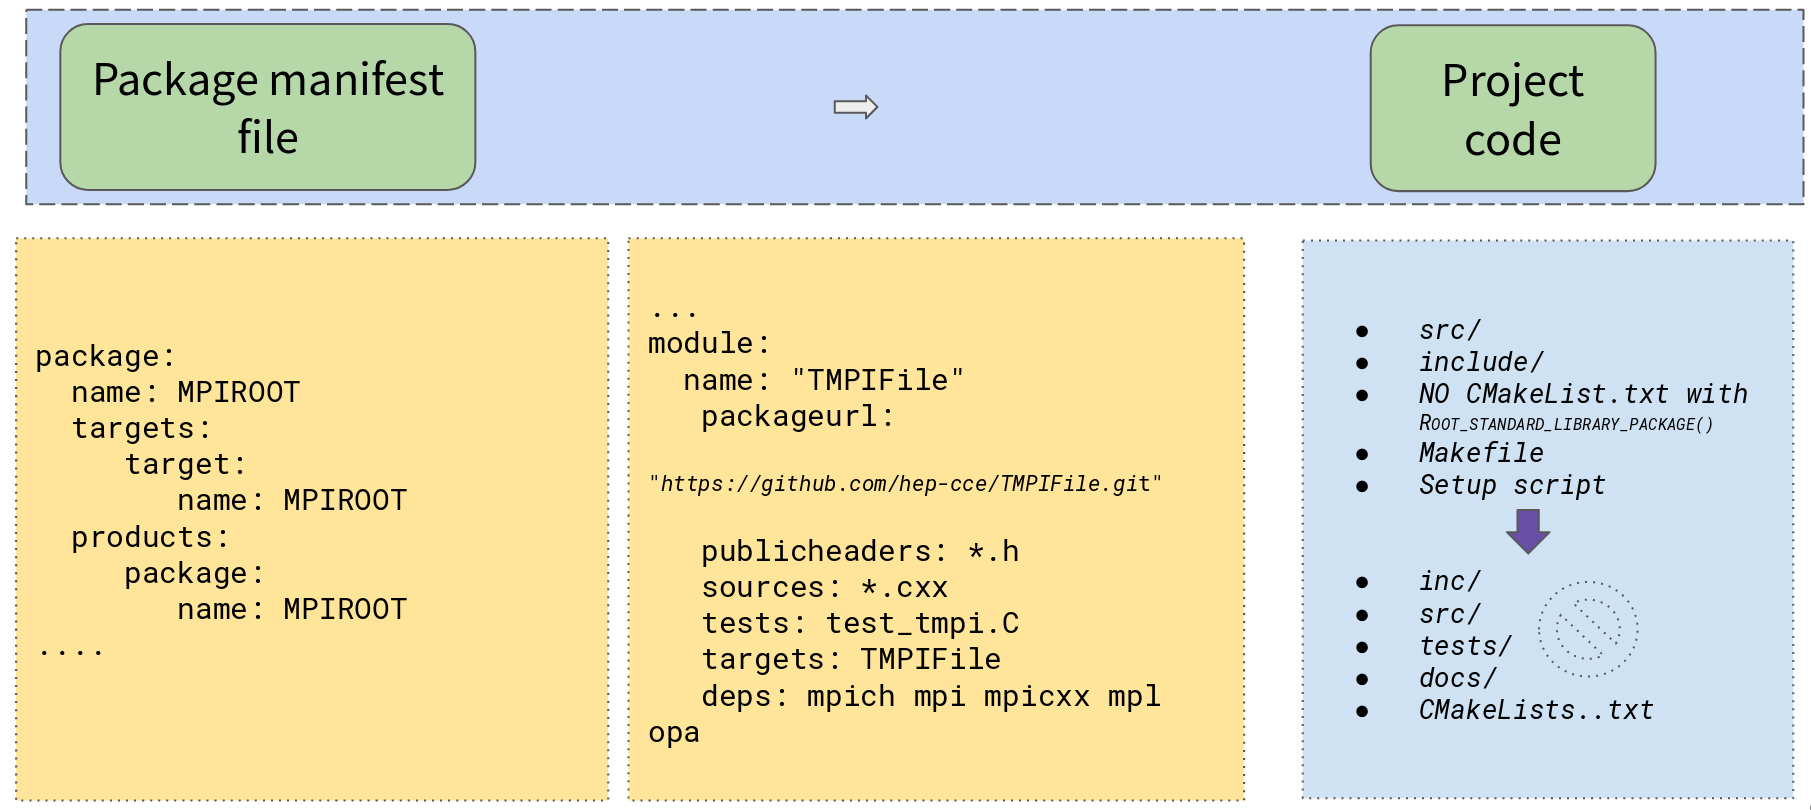
\includegraphics[width=1.0\linewidth]{picture/2.png}
%\caption{}
%\label{interp}
%\end{figure}

%\begin{figure}
%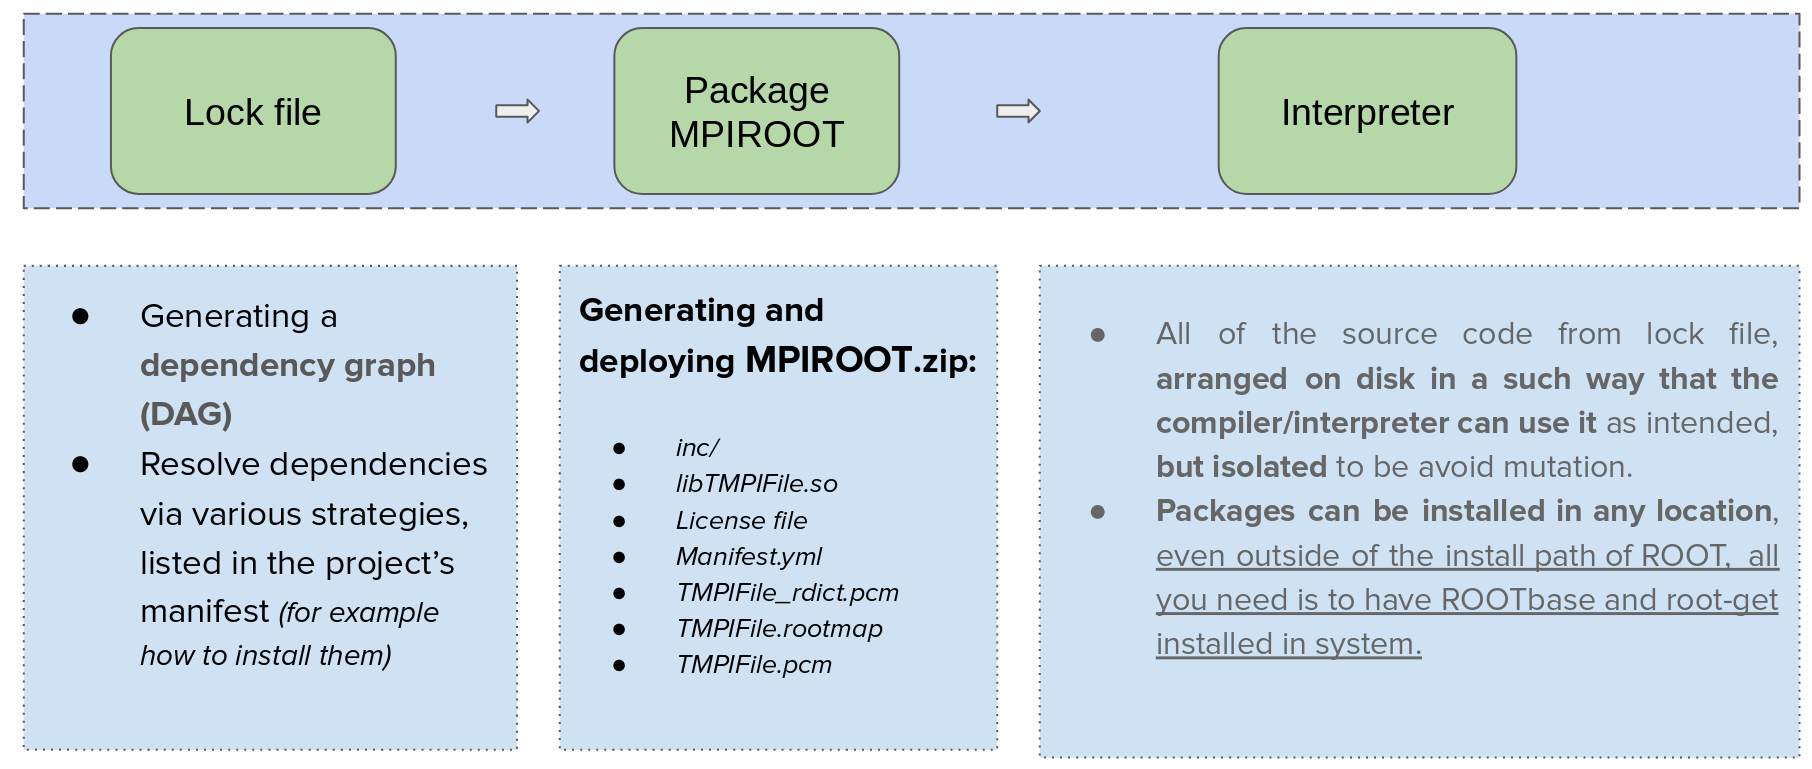
\includegraphics[width=1.0\linewidth]{picture/4.png}
%\caption{}
%\label{interp}
%\end{figure}

\section{Package manager design prototype}

As a part of the package manager prototype was defined two different future work areas: ROOT Base package as a fundamental part of ROOT, and development of ROOT package management tool.

\subsection{Evolving “Minimal ROOT” to “ROOT Base”}

While generating the ROOT libraries dependency graph, we can quickly notice that it is hard to visualize a small core of ROOT as desired for our ROOT Base package. % We need to start to work on modularization of a ROOT package from the bottom to the top, trying to build new ROOT modular system step by step.

ROOT's build system provides a “minimal ROOT” option that is supposed to build only the essential functionality of ROOT required for basic I/O operations. At the outset of this project, nearly fifty components were built when this \textit{minimal} option was enabled; we believe that “Minimal ROOT” has migrated away from its original goal of being only a \textit{core-like} ROOT. We have worked to trim the minimal build down include three components, Core, I/O, and Cling libraries, and the smallest number dependencies required.

Our \textit{ROOT Base} is formed by taking these three components and their transitive dependencies using CMake-based introspection.
% TODO(brian): I don't understand why the next sentence belongs in this paragraph...
% Oksana: I totally agree!
% TCling, an interpreter interface in the ROOT Core library, provides an API, to contribute a set of operations with a ROOT interpreter allowing operations with mangled names for methods of classes, ROOT headers auto-parsing and libraries autoloading and also will play an important role as an interface to the ROOT package manager.

\subsection{ROOT Package Manager - root-get}
\subsubsection{Design specifications}
A package manager is a standalone tool for managing the distribution of software code.  Package managers are classified into the three sub-types: operation system package manager (OSPM), language package manager (LPM) and project or application dependency manager (PDM). We will focus on PDMs since operation system package managers and language package managers are out of the scope of the goal of this paper. A project dependency manager is an interactive system for managing the source code dependencies of a single project written in a particular language offering multiple operations on the dependent code of the project. Project dependency manager's output is a self-contained and precisely reproducible source tree that acts as the input to a compiler or interpreter. It could also be referred to as a \textit{compiler, phase zero} \cite{pdm}.

The ROOT package manager best fits as a project dependency manager. Since ROOT has incorporated C++ interpreter in its code source, the project dependency manager's functionality could be expanded to be made available at both ROOT build time and runtime. This enables the possibility to develop hooks allowing one to use the package manager during ROOT runtime. Using the package manager during runtime is where a pure CMake implementation would fall short as CMake does not have any support for steps happening after build or install time.

%NOTE(bbockelm): I don't understand the point of this paragraph.  It doesn't seem to add much - can we just delete it?  If we bring it back, we should say more about how we 

%A ROOT package management system can manage the package lifetime to ensure sustainability transparently. The role of the ROOT package manager is to reduce coordination costs by automating the process of downloading and building all of the dependencies for a project required for users, experiments or the entire community while avoiding complex dependency conflicts. When a project's packages have requirements that conflict with one another, it creates a situation often referred to as "dependency hell." Improper project dependency management is a reason for the ``dependency hell situation which could be a reason of lengthy downloads and decreasing the portability of the software. Dependency hell is a common problem found in software that is built using an add-on software package. Dependency hell can take many forms and occur for many reasons, such as the need to install add-on software libraries, the need for long chains of installations, problems with a different program, the creation of circular dependencies and more. Often, rather than "reinventing the wheel," software should be designed to take advantage of other software components that are already available or have already been designed and implemented for use elsewhere.

An essential part of the ROOT package manager's design is the use of C++ modules technology.
% I don't understand the below - are Clang C++ modules not C++ modules?
% there is three different implementations of c++ modules: Clang, gcc and Visual Studio. 
C++ modules can optimize header parsing, providing a possibility of loading on-demand code. In this article, we will be talking about ROOT C++ modules, which are C++ modules generated by internal Clang compiler, available in ROOT and heavily relying on the Clang implementation of C++ modules.

% How do `ROOT runtime C++ module' differ from Clang C++ modules?  Not defined!
% What is your definition of separable?
Since ROOT has own interpreter, ROOT C++ modules can be used during ROOT runtime and in this case we will reference them as a ROOT runtime C++ modules or implicit C++ modules. We will reference ROOT C++ modules used during ROOT compile time, as explicit C++ modules. 

ROOT implicit C++ modules solve the limitation that the ROOT compiled header (PCH) is non-separable or non-modular and PCH must be regenerated each time when a new ROOT library is configured. Implicit C++ modules are available in the ROOT 6.16.00 release binaries, as a technology preview, which allows us to test them during the package manager development.

% NOTE(bbockelm): I'm not sure this paragraph is saying anything not in the prior sections?
%Before developing the ROOT package manager, one of the last tasks to be solved is to provide improved ROOT modularity for its build system and simplifying dependencies to allow a smaller ROOT Base package and other ROOT components. It will also allow users to benefit possibilities to combine various feature builds without rebuilding the whole ROOT from the beginning and provide a "lazy install" service for ROOT.

\subsubsection{Requirements for the ROOT package manager}

The ROOT package manager should satisfy a set of functionality requirements expected by ROOT users. That includes more comprehensive sets of operations with the manifest files, sanity checks of the content of the manifest files, and execution commands. At the current stage of research, it is essential to define minimum requirements for functionality of the package manager, definitions of entities (such as  a component and package), and the format of the manifest file. 

For our purposes, the minimal requirement for the ROOT package manager is to be able to define and resolve dependencies and versions through the manifest of the package. These should be done either for ROOT packages or its external dependencies. 

Ideas for future extensions are inspired by the functionality of Swift Package Manager \cite{swiftpm}, which is supported by a large  community:
\begin{enumerate}
\item Automated testing; 
\item Support of cross-platform packages;
\item Support for operating system package managers (homebrew, etc.);
\item Support for version control system;
\item Standardized licensing;
\item Introduction of a package index;
\item Importing dependencies by source URL;
\item Component inter-dependency determination;
\item Complex dependency resolution.
\end{enumerate}

Using benefits from the introduction of C++ module infrastructure for ROOT, we followed the ideas of Swift Package Manager and implemented a standalone tool - `root-get' which provides functionality meeting the a minimal requirements described above.


\subsubsection{root-get prototype}

We have implemented a dependency management tool for ROOT (Figure 2) called `root-get'. It consists of the multiple modules that provide the desired package management functionality:
\begin{enumerate}
\item \textbf{Analyzer} defines environment variables, checks if there are existing manifest/package YAML files, and sets up the environment (discovering the location of components and packages and preparing for the manifest’s generation).
\item \textbf{Generator} encapsulates the ROOT CMake functions for generating information for  manifest files. It allows one to configure ROOT modules and packages outside of ROOT using special CMake files containing the definitions about ROOT CMake functions and ROOT external dependencies.
\item \textbf{Downloader} is a set of helper routines for downloading packages from Github or other location.
\item \textbf{Resolver} is a module that provides a package database generation and resolution of dependencies via generated direct acyclic graph (DAG).
\item \textbf{Builder} is a module that provides ROOT packaging scripts.
\item \textbf{Integrator} is a module that provides installation and deployment routine for ROOT packages. 
\end{enumerate}

% NOTE: Is there really nothing else we can say about the prototype?  Seems strange to spend 4 pages talking about requirements and semantics but almost nothing about the work we did....

A root-get is using the generic approach, existing for all "package managers" and works directly with the source code of components. Manifest files, in this case, are usually the files generated by static code analysis tools or provided by the user. The core part of package manager workflow is a "lock file". It is a file containing the project dependencies that are generated directly from manifest files. The expected result after package manager operations is a delivery of the set of artifacts: compiled source code and its dependencies, which can serve as a direct “input” to the interpreter and usually generated from lock file.

All compiled source code, declared by the lock file should be arranged on disk in such way that the compiler or interpreter can use it as intended, but it will be still isolated to avoid mutation. ROOT components arranged as a set of packages could be installed in any location, even outside of the install path of ROOT. All necessary components for the successful setup are ROOT Base installation and root-get installed in the system.

ROOT Base together with root-get is capable of providing proper infrastructure for custom ROOT distribution and natural extension of ROOT functionalities, which includes the possibility to build any ROOT components and also plug-in custom user components.

\begin{figure}[!h]
  \centering
  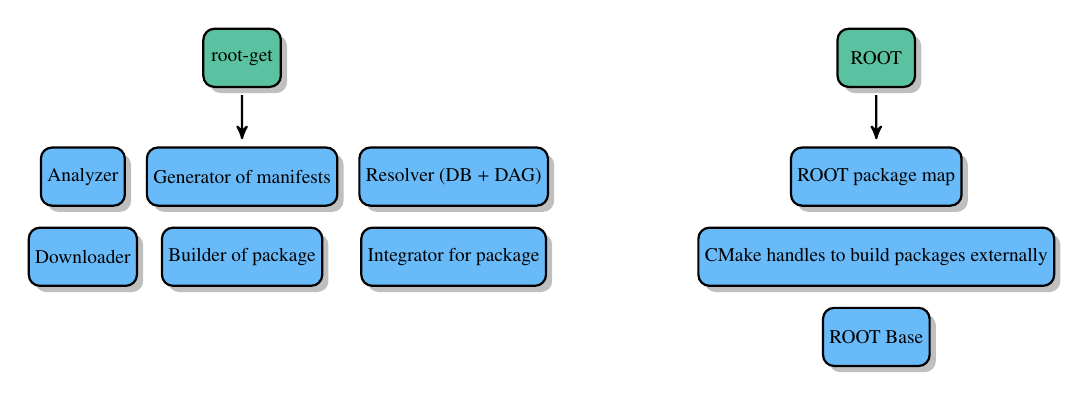
\begin{tikzpicture}[outer sep=0.05cm, node distance=0.8cm, scale=0.7, transform shape]
        
    \node[model, fill=my_green, name=rootget] (rootget) {root-get};
    \node[model, fill=my_green, name=root, right=10cm of rootget] (root) {ROOT};
    \node[model, fill=my_lightblue, name=gen, below=1cm of rootget] (gen) {Generator of manifests};
    \node[model, fill=my_lightblue, name=anal, left=0.3cm of gen] (anal) {Analyzer};
    \node[model, fill=my_lightblue, name=resolv, right=0.3cm of gen] (resolv) {Resolver (DB + DAG)};
    \node[model, fill=my_lightblue, name=downl, below=0.3cm of anal] (downl) {Downloader};
    \node[model, fill=my_lightblue, name=build, below=0.3cm of gen] (build) {Builder of package};
    \node[model, fill=my_lightblue, name=int, below=0.3cm of resolv] (int) {Integrator for package};
    \node[model, fill=my_lightblue, name=rpm, below=1cm of root] (rpm) {ROOT package map};
    \node[model, fill=my_lightblue, name=cmake, below=0.3cm of rpm] (cmake) {CMake handles to build packages externally};
    \node[model, fill=my_lightblue, name=rb, below=0.3cm of cmake] (rb) {ROOT Base};

    \draw[line, ->] (rootget.south) -- (gen);
    \draw[line, ->] (root.south) -- (rpm);

  \end{tikzpicture}
  \caption{Components of root-get prototype.}
  \label{fig:InformationFlow}
\end{figure}

\section{Conclusions}

We have defined the desired functionality for a package management ecosystem for ROOT. We defined a minimal and extended set of requirements for the ROOT package manager. These ideas have been adopted into a preliminary prototype that can download and install packages. As it matures, the prototype will be connected directly to the ROOT runtime and serve as a runtime dependency management tool.\\

{\small This work has been supported by U.S. National Science Foundation grants OAC-1450377, OAC-1450323, and PHY-1624356.}

\begin{thebibliography}{plain}

\bibitem{root}
R. Brun, F. Rademakers, \textit{ROOT - An Object Oriented Data Analysis Framework}, Nucl. Inst. \& Meth. in Phys. Res. A  \textbf{389} (Proceedings AIHENP'96 Workshop,1997).

\bibitem{rootcxxmodules}
V. Vassilev. \textit{Optimizing ROOT's Performance Using C++ Modules. Journal of Physics: Conference Series}, \textbf{898}. 10.1088/1742-6596/898/7/072023. (2016)

\bibitem{rootgit}
GitHub.\textit{GitHub - root-project/root: The official repository for ROOT: analyzing, storing and visualizing big data}, Available at: https://github.com/root-project/root. [Accessed 03 December 2018]. (2018)

\bibitem{cxxmodules}
\textit{Modules — Clang 8 documentation}. Available at: https://clang.llvm.org/docs/Modules.html. [Accessed 30 November 2018]. (2018)

\bibitem{swift}
GitHub. \textit{GitHub - apple/swift: The Swift Programming Language}. Available at: https://github.com/apple/swift. [Accessed 30 November 2018]. (2018)

\bibitem{yaml}  Yaml.org. \textit{YAML Ain’t Markup Language (YAML™) Version 1.2.} [online] Available at: http://yaml.org/spec/1.2/spec.html [Accessed 6 Mar. 2019].

\bibitem{pdm}
Medium. \textit{So you want to write a package manager – Sam Boyer – Medium}. Available at: https://medium.com/@sdboyer/so-you-want-to-write-a-package-manager-4ae9c17d9527. [Accessed 30 November 2018]. (2018)

\bibitem{swiftpm}
GitHub.\textit{GitHub - apple/swift-package-manager: The Package Manager for the Swift Programming Language.} Available at: https://github.com/apple/swift-package-manager. [Accessed 30 November 2018]. (2018)



\end{thebibliography}

\end{document}

% end of file template.tex

<div id='footer'><table width='100%'><tr><td class='right'><a href='http://fusioninventory.org/'><span class='copyright'>FusionInventory 9.1+1.0 | copyleft <img src='/glpi/plugins/fusioninventory/pics/copyleft.png'/>  2010-2016 by FusionInventory Team</span></a></td></tr></table></div>